\section{Ziel}
\label{sec:Ziel}
Der Frank-Hertz-Versuch zählt zu den Elektronenstoßexperimenten. 
Diese werden genutzt, um die Struktur der Elektronenhülle eines Atoms genauer zu erforschen.
Ziel ist es, die Anregungsenergie eines Quecksilberatomes zu bestimmen, die Energieverteilung der stoßenden Elektronen zu untersuchen, sowie die Ionisierungsenergie von Quecksilber zu beziffern.

\section{Theorie}
\label{sec:Theorie}
\subsection{Anregung eines Hg-Atoms}
Zur Bestimmung der Anregungsenergie eines Quecksilberatoms wird dieses mit Elektronen bestimmter Energie beschossen.
Die Elektronen übertragen durch Stoßprozesse ihre Energie auf das Atom und versetzen es in einen angeregten Zustand.
Aus den Informationen des Energieverlustes der stoßenden Elektronen können Rückschlüsse auf die Anregungsenergie $E_\mathup{a}$ gezogen werden. 
Stoßen Hg-Atom und Elektron unelastisch, so nimmt das Atom die Energie
\begin{equation}
	\label{eq:E_a}
	\frac{m_\mathup{e} v_\mathup{vor}²}{2}-\frac{m_\mathup{e} 	v_\mathup{nach}²}{2}=E_1-E_0=E_\mathup{a}
\end{equation}
auf.
$m_\mathup{e}$ bezeichnet die Masse der stoßenden Elektronen, $v_i$ ihre Geschwindigkeit vor und nach dem Stoß, $E_0$ die Energie des Hg-Atoms im Grund- und $E_1$ die Energie im ersten angeregten Zustand. 
Nach einer Relaxationszeit von $t \approx \SI{10e-8}{\second}$ geht das Hg-Atom wieder in den Grundzustand über und emittiert ein Lichtquant der Energie
\begin{equation}
	h \nu =E_1-E_0.
\end{equation} 
Damit ein unelastischer Stoß zustande kommt muss für die Energie der stoßenenden Elektronen die Bedingung $E_\mathup{e} \geq E_\mathup{a}$ gelten. 
Wird diese nicht erfüllt stoßen Elektron und Atom elastisch. 
Es kommt aufgrund des großen Massenunterschiedes zu einer geringen Energieabgabe.
%von 
%\begin{equation}
%	\Delta E=\frac{4m_\mathup{e}M}{(m_\mathup{e}+M)²}\cdot 		E_	\mathup{e} \approx 1,1\cdot 10⁻⁵ E_\mathup{e}
%\end{equation}
Dieser kleine Energiebetrag ruft nur eine Richtungsänderung in der $z$-Komponente des Elektrons hervor, führt jedoch nicht zu einer Anregung der Atome.

\subsection{Idealisierte Franck-Hertz-Kurve}
\begin{figure}
	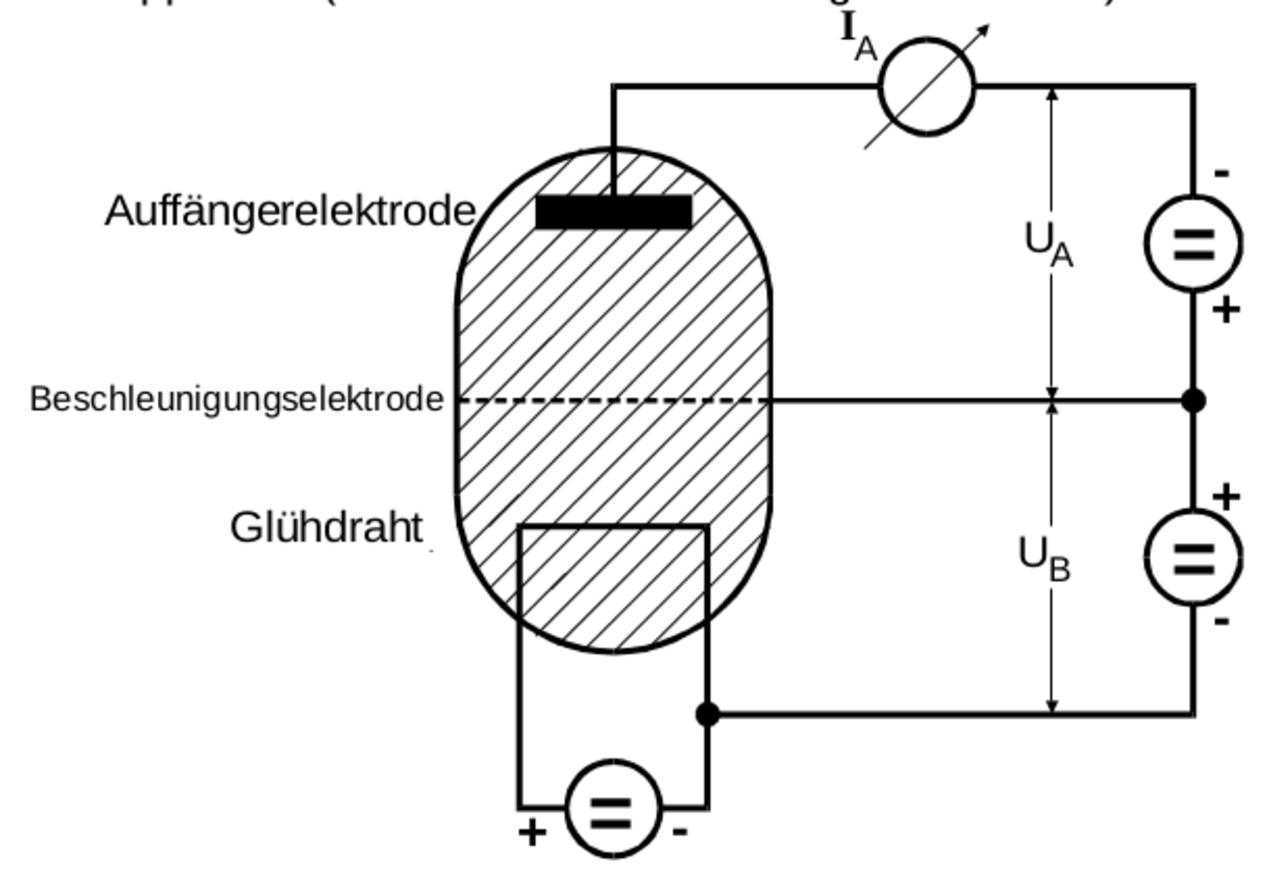
\includegraphics[width=0.5\textwidth]{Bilder/Aufbau.pdf}
	\caption{Grober Aufbau des Franck-Hertz-Versuchs.}
\end{figure}
In einem evakuierten Gefäß befindet sich ein Tropfen Quecksilber (Hg), der teilweise verdampft. 
Abhängig von der Umgebungstemperatur $T$ bildet sich ein Gleichgewichtsdampfdruck $p_\mathup{sät}$ aus. 
Ein heißer Glühdraht dient als Elektronenlieferant.
Durch eine gitterförmige Beschleunigungselektrode (BE) mit positiver Beschleunigungsspannung $U_\mathup{B}$ wird den Elektronen eine Energie von 
\begin{equation}
	e U_\mathup{B}=\frac{m_\mathup{e}v_\mathup{vor}²}{2}
\end{equation}
zugeführt. 
Erreichen die Elektronen die Auffängerelektrode (AE) lässt sich ein Auffängerstrom $I_\mathup{A}$ messen. 
Elektronen treffen jedoch nur auf die AE, wenn sie genug Energie besitzen um zuvor deren Bremsfeld, erzeugt durch die Spannung $U_\mathup{A}$, zu überwinden. 
Nur Elektronen mit 
\begin{equation}
	\frac{m_\mathup{e}}{2}v_\mathup{z}² \geq e U_\mathup{A}
\end{equation}
passieren diese Hürde -- die restlichen Elektronen kehren zur BE zurück.
Zur Bestimmung der Anregungsenergie wird die zuvor beschriebene Gegenfeldmethode benutzt. 
Während die Elektronen sich durch das Gefäß bewegen stoßen sie mit den Hg-Atomen zusammen. 
Das Beobachten des Auffängerstroms $I_\mathup{A}$ gibt Aufschluss über die Anregungsenergie.
Ein Erhöhen von $U_\mathup{B}$ lässt den Strom ansteigen, da immer mehr Elektronen die AE erreichen.
Sobald die Elektronen eine Energie aufweisen, die gleich der Anregungsenergie ist, geben sie diese durch Stöße an die Hg-Atome ab. 
Danach reicht ihre Energie nicht mehr aus, um das Gegenfeld zu passieren - $I_\mathup{A}$ fällt rasant ab.
Starkes Erhöhen von $U_\mathup{B}$ führt den Elektronen so viel Energie zu, dass mehrere Stöße ermöglicht werden. 
Die Abstände der Maxima $U_1$ in Abbildung \ref{fig:id} entsprechen der Anregungsenergie des Hg-Atoms im ersten Zustand:
\begin{equation}
	U_1=\frac{1}{\epsilon_0}{(E_1-E_0)}.
\end{equation}
\begin{figure}
	\centering
	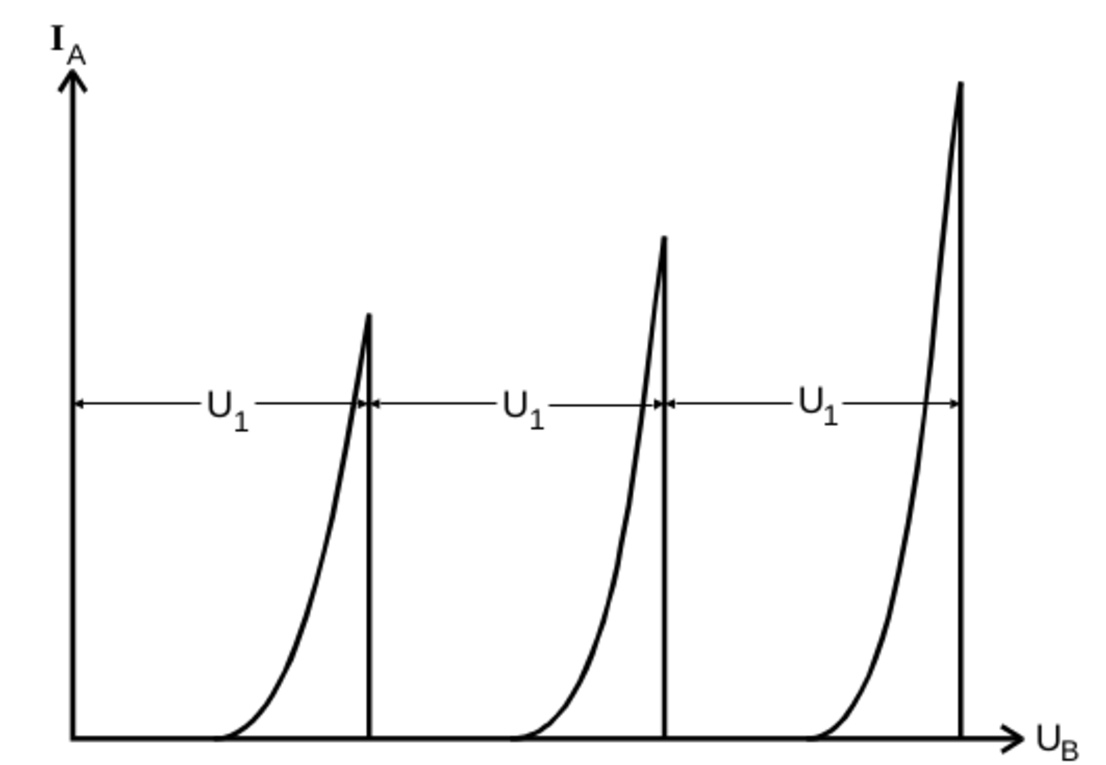
\includegraphics[width=0.5\textwidth]{Bilder/Kurve_Theo.pdf}
	\caption{Theoretischer - idealisierter - Kurvenverlauf des Auffängerstroms $I_\mathup{A}$.}
	\label{fig:id}
\end{figure}
Der tatsächliche Kurvenverlauf weicht vom idealen etwas ab, da einige messbedingte Nebeneffekte auftreten.

\subsubsection{Nebeneffekte}
\begin{enumerate}
\item{Das Kontaktpotential}

Die eingestellte Spannung $U_\mathup{B}$ entscheidet sich von der tatsächlichen Beschleunigungsspannung. 
Grund dafür sind die Potentiale $\varphi_\mathup{D}$ und $\varphi_\mathup{BE}$ , d.h. die Austrittsarbeit der Elektronen aus verwendetem Glühdraht und der Beschleunigerelektrode. 
Diese unterscheiden sich dank unterschiedlichem Material.
Die Effektivspannung ist um den Betrag des Kontaktpotentials K herabgesetzt und die Kurve deswegen verschoben.
\begin{equation}
	U_\mathup{B,eff}=U_\mathup{B}-\frac{1}{\epsilon_0}(\Phi_	\mathup{BE}-\Phi_\mathup{D}=U_\mathup{B}-K
\end{equation}
\item{Energiespektrum der Elektronen}

Nach der \textsc{Fermi}-\textsc{Dirac}-Verteilung weisen die Leitungselektronen eines Metalls ein Energiespektrum auf und besitzen damit unterschiedliche Anfangsgeschwindigkeiten.
Das hat zur Folge, dass die Kurvenmaxima sich langsamer ausbilden und flacher werden. 
Außerdem ist kein unstetiger Abfall der Kurve auf ein Stromminimum von $I_\mathup{A}=0$ zu beobachten.
Richtungsänderungen eventueller elastischer Stöße zu einer Verbreiterung des Kurvenverlaufs, sofern diese zwischen BE und AE stattfinden. 
\item{Dampfdruck}

Für die mittlere freie Weglänge $\overline{w}$ muss $\overline{w} < a$ mit dem Abstand $a$ zwischen BE und AE gelten, um die Wahrscheinlichkeit unelastischer Stöße zu maximieren. 
$\overline{w}$ ist über den Dampfdruck $p_\mathup{sät}$ steuerbar. Dieser wird über die Temperatur $T$ eingestellt. 
\begin{equation}
	\overline{w}=\frac{0,0029}{p_\mathup{sät}}
	p_\mathup{sät}(T)=5,5\cdot 10⁷\exp{-\frac{6876}{T}}, [p_\mathup{sät}=\si{\milli\bar}, [\overline{w}]=\si{\centi\meter}.
\end{equation}
In einem bestimmten Temepraturbereich ist die Stoßwahrscheinlichkeit optimal.
Ein kleinerer Druck führt zu einer geringen Stoßwahrscheinlichkeit, ein größerer Druck führt zu vielen elastischen Stößen.
\end{enumerate}
